%latex report

\documentclass[a4paper,11pt]{article}
\usepackage{times}
\usepackage{graphicx}
%\usepackage{amsmath}
\usepackage{natbib}
\usepackage[top=2.54cm, bottom=2.54cm, right=1.27cm, left=1.27cm]{geometry}
\begin{document}


\title{Physics Behind the Simulation: A CS296 Group 31 Report.}

\author{Sanchit Garg\\ 110050035\\	\texttt{sanchitgarg@cse.iitb.ac.in} \and
		Ravi Kumar Roshan\\ 110050033\\ \texttt{sraviroshan@cse.iitb.ac.in}
		}

\date{10 April, 2013}

\maketitle


\section{Introduction}
A Rube Goldberg machine, contraption, invention, device, or apparatus is a deliberately over-engineered or overdone machine that performs a very simple task in a very complex fashion, usually including a chain reaction. The expression is named after American cartoonist and inventor Rube Goldberg (1883–1970). ~\cite{wiki}%////Wikipedia

This is a small Project Report about the simulation and contraption using C++ Simulator engine Box2D under the CS296 Lab Course.

Here we first describe the design of the simulation followed by its timing and Profiling issues.

\section{Design}
First we start with implemented design. Design is very simple. Implemented and original design are almost same. We then describe some minor changes we have done in original design.~\cite{lt}
\subsection{Implemented Design}	

\begin{center}
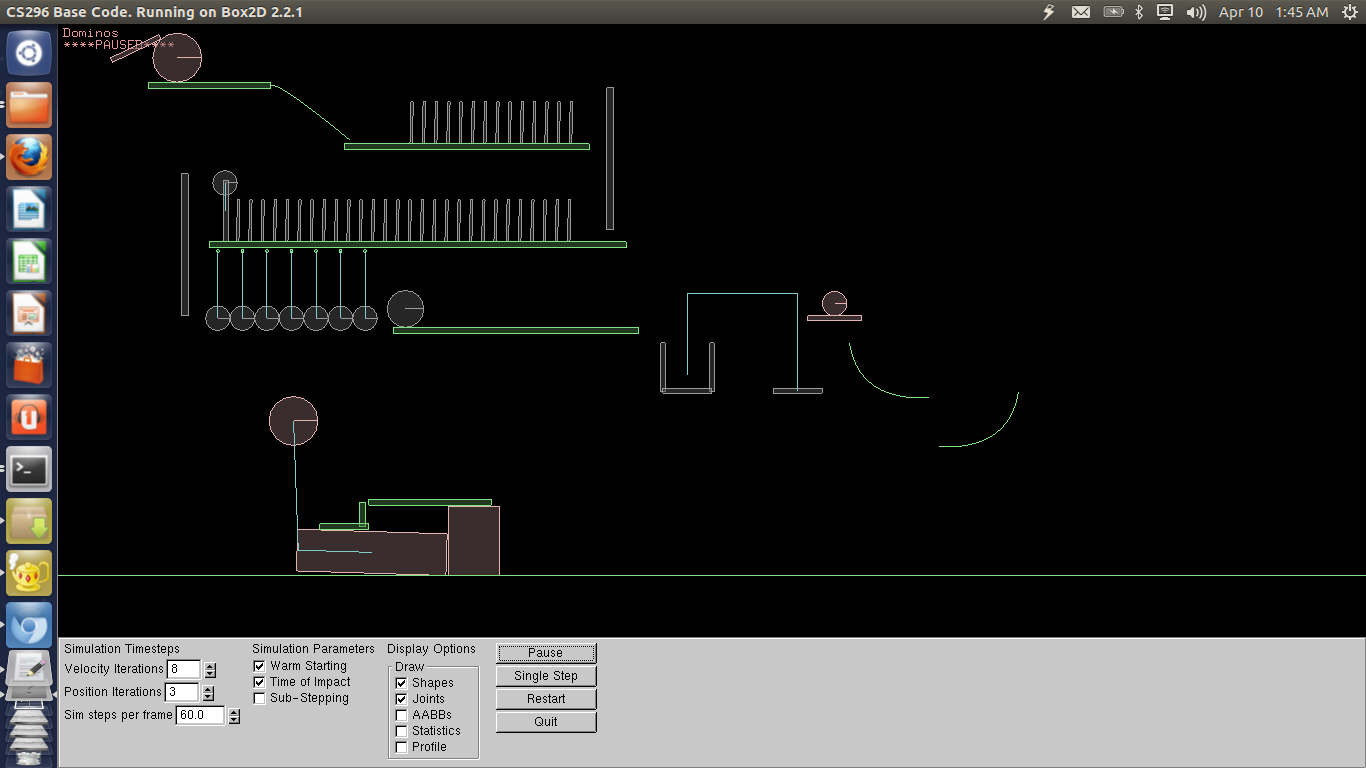
\includegraphics[scale=0.3]{./doc/photo1.png}
\begin{center}
Fig.1
\end{center}
\end{center}

First a Motored plank. It starts revolving and strikes a ball resting on a platform. 
This ball rolls down from a slope and hits the train of Dominos standing on horizontal Platform. Dominos start falling. There is a rotating shaft near the end of this domino train. It gets hit by the dominos. This shaft while rotating hits another train of Dominos standing on another horizontal platform just below the first one. On the end of this domino train there is another rotating shaft which do the same purpose that as of the previous one. This rotates on hit by dominos. On the way of its rotaion Newton's Cradle is kept. Shaft hits the Newton's Cradle. Near the end of the Cradle a ball is kept. This  ball get struck by the cradle and rolls horizontally and finally enters in pully system. There is a Bucket(open box) into which the ball falls. When this ball falls, the bucket becomes heavier and starting coming dowm and as a result the other side of pulley which is connected by a horizontal plank, starts moving up and make rotates the another horizontal platform. There is a ball resting on this platform which falls down due to movement of platform. This ball follows a zig-zag path on two curves and falls on ground and moves towards a piston. Finally the ball hits the piston. On the mouth of piston there is a block attached with a balloon. This balloon is basically a ball whose gravity is reversed. Ball coming towards the piston hits and balloon moves up along with block.~\cite{kk}

\subsection{Original Design}
There are 3 changes apart from body's structure :
\begin{center}
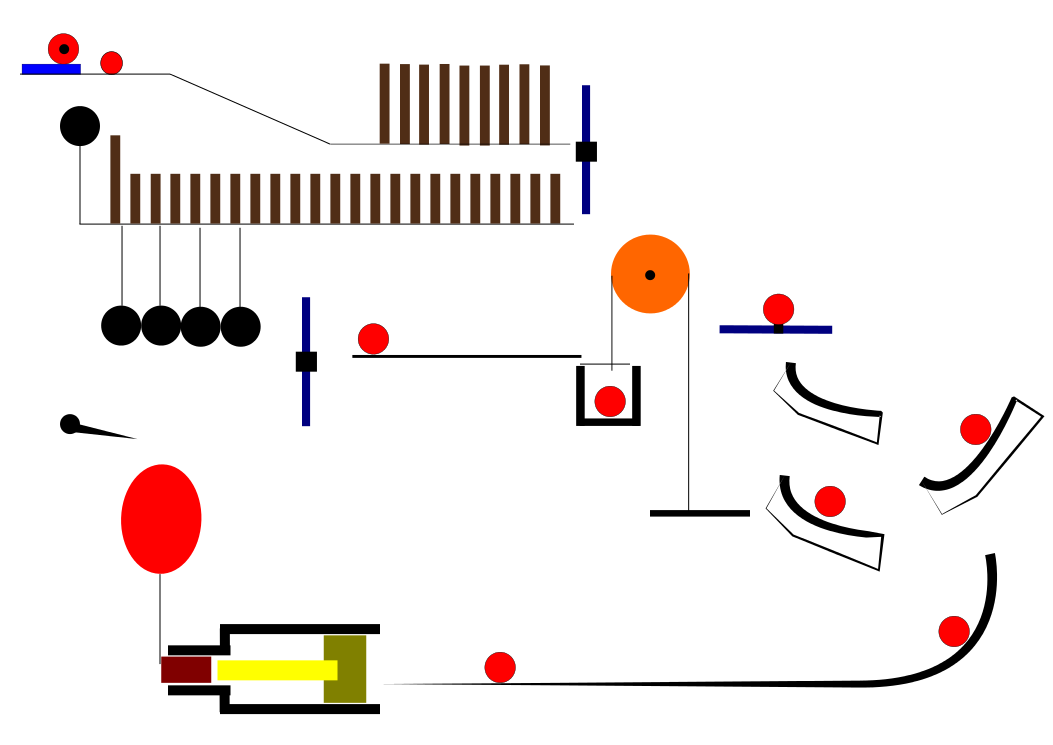
\includegraphics[scale=0.3]{./doc/idea.png}
\begin{center}
Fig.2
\end{center}
\end{center}

\begin{itemize}
\item {Motored Plank}
\begin{description} Instead of motored plank We thought of a revolving ball which is in contact with a plank. As ball rotates plank moves and hit a ball and continue.
\end{description}

\item {Second Revolving Shaft}
\begin{description} Instead of second revovling shaft We planned that at the end of the second dominos train there is a inverted pendulum standing and on hit it moves down and starts the motion of Newton's Cradle.
\end{description}

\item{Bursting of Balloon}
\begin{description} We thought that as the balloon rise it would come into the contact of a pointed thing and will burst.
\end{description}
\end{itemize}

\subsection{Interesting Features}
\begin{itemize}
\item {Newton's Cradle}
\begin{description} Newtons Cradle may look like interesting but in simulation the exact effect of it has not achieved i.e only end balls move.
\end{description}

\item {Rising Balloon}
\begin{description} Rising Balloon (acieved by reversing its gravity) may look like interesting.
\end{description}
\end{itemize}


\section{Timing Analysis}

\subsection{Observations}

\begin{enumerate}

\item{Plot1: Loop time increases with no of iterations.}
\begin{description}
It is obvious. As no. of iterations increases the time taken to simulate more steps increases.
\end{description}


\begin{center}
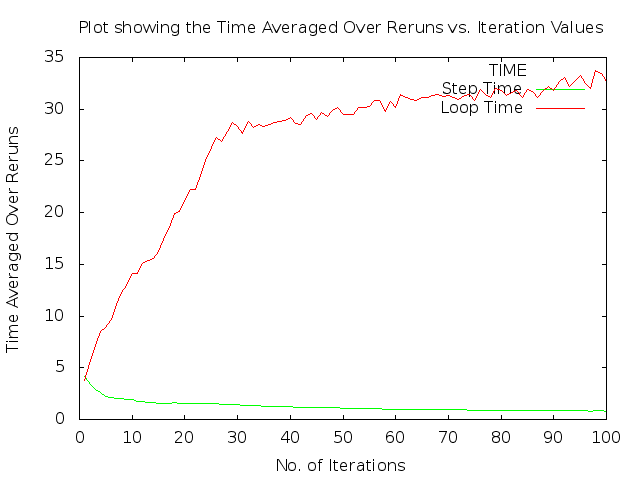
\includegraphics[scale=0.3]{./plots/g31_plot01.png}
\begin{center}
Fig.3 Plot01 : step and loop time averaged over all reruns for various iteration values
\end{center}
\end{center}

\item{Plot1: Graph segmented into two linear parts for loop time for both load and no-load graph
\begin{enumerate}
\item{0-30 :}
	higher slope, less deviation from linear; and
\item{30-100 :}
	lesser slope, more fluctuations from being linear.
\end{enumerate}}

\begin{description}
As the no. of iteration increases more work has to be done by the system, so system provides more resources to this and gives priority to this process. Hence more work is done by the system to run the process and hence simulation runs relatively faster so average time decreases.
We have run for iteration no. 5000,10000 and observed the avg. step time decreases.
\end{description}

\begin{center}
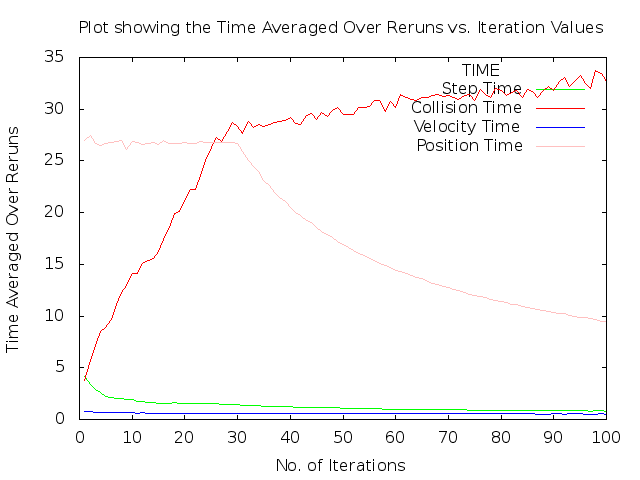
\includegraphics[scale=0.3]{./plots/g31_plot02.png}
\begin{center}
Fig.4 Plot02 : step,collision,position and velocity update time averaged over all reruns for various iteration values
\end{center}
\end{center}

\item{Plot2: Times(Step, Velocity, Position, Colllision) for various iterations averaged over reruns decreases as iteration value increases.}
\begin{description}
It may be possible that as simulation proceeds ahead the simulation steps are performed faster or the amount of work the simulation is doing get decreased in further steps. Or it may be possible also that initially the application requires some amount of time to stablize the process and hence takes more time in the beginning than afterwards. As a result time for single step averaged over 100 reruns decreases as no. of iteration value increases. Also if we run simulaiton for higher values let say 10000 or 50000 for various reruns, we can verify the trend. It is due to compiler optimison also. As no. of iteration increases, amount of work also increases. Same work is not computed many times by compiler. So averaged time decreases.
\end{description}

\begin{center}
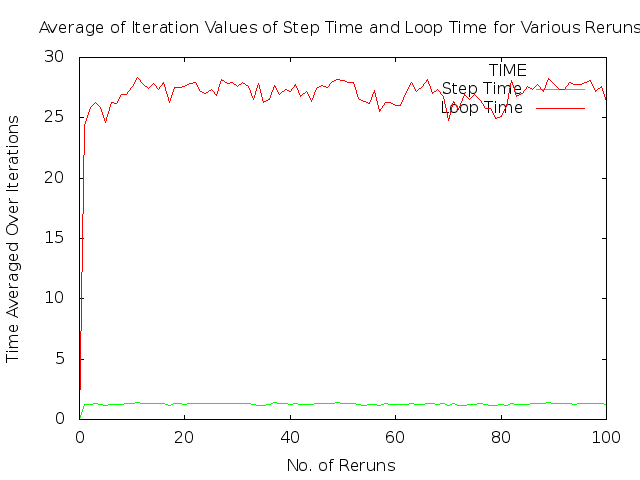
\includegraphics[scale=0.3]{./plots/g31_plot03.png}
\begin{center}
Fig.5 Plot03 : step and loop time averaged over all iterations for various rerun values
\end{center}  \and


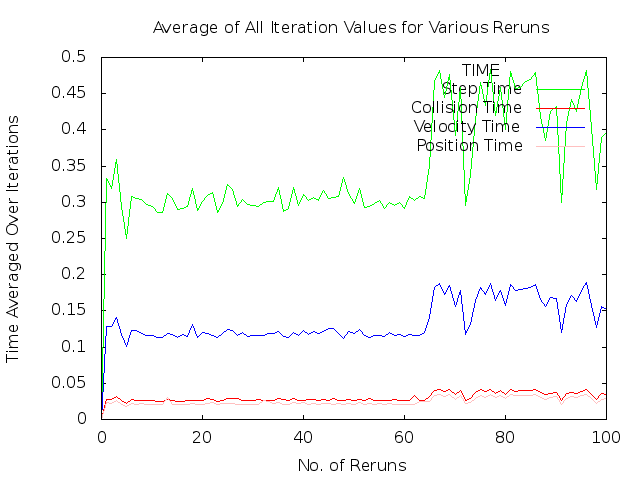
\includegraphics[scale=0.3]{./plots/g31_plot04.png}
\begin{center}
Fig.6 Plot04 : step,collision,position and velocity update time averaged over all iterations for various rerun values
\end{center}
\end{center}

\item{Plot3 and Plot4 as load increases these plots fluctuate readily as compared when load is low and relative values is large in first one as compared to second}
\begin{description}
As more and more programs run on machine, the process of memory and other resource allocation and usage fluctuates more. So as the system get more and more busy, efficiency and performence of the processes running on the machine is affected and get degraded.
\end{description}


\begin{center}
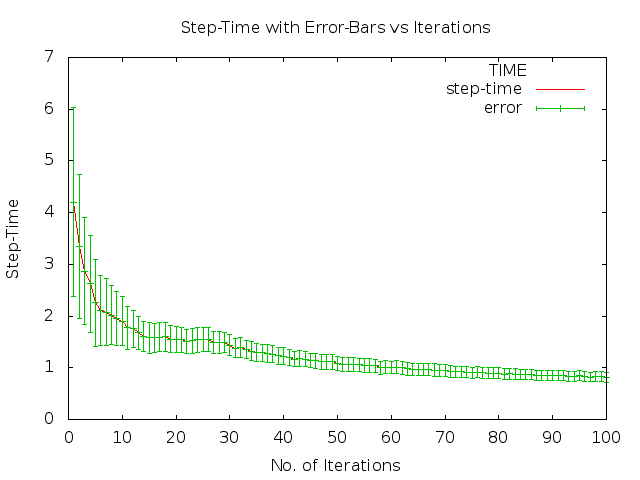
\includegraphics[scale=0.3]{./plots/g31_plot05.png}
\begin{center}
Fig.7 Plot05 : step time for various iteration values with error bars
\end{center}
\end{center}

\item Plot5: Comparing error bars
\begin{enumerate}
\item{Length of error bars corresponding for the values is relatively low when load is low as compared when load is high.}
\begin{description}
As described above, as the machine is highly loaded with so many processes, the fluctuations of time calculation and other processes are very high and there is very high chances of error in calculations and it happens as we compare the two plots.
\end{description}
\item{Window of error bar decreases as we increase no. of iterations.}\\
As no. of datasets increases in a sample, error(Standard Deviation) decreases. This can also be inferred from Central Limit Theorem. 
\end{enumerate}


\begin{center}
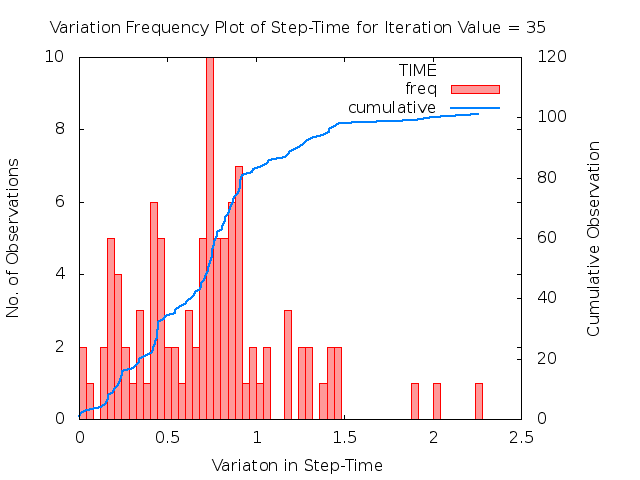
\includegraphics[scale=0.3]{./plots/g31_plot06.png}
\begin{center}
Fig.8 Plot06 : frequency values as a bar graph and the cumulative frequency values as a curve
\end{center}
\end{center}

\item{Plot6: Frequency plot is baised towards left.}
\begin{description}
As in plot2 we saw that no. of low averaged value is more than high averaged value (because step time decreases readily in beginning and then gradually decreases) therefore we can say and observes that frequency plot is baised towards left.
\end{description}
\end{enumerate}


\section{Profiling}
A profiler is used to identify what are the parts of your code are taking the maximum time. This helps in identifying parts of your code that can be optimized. Here below is the profiling done first with optimization i.e with release mode on and second with debugging mode on. For profiling we have used perf tool.

\subsection{Observations}
Analysis has beem done on the iteration no. 200, 1000 and 5000.
\begin{itemize}
\item{For Iteration no. 200}
\begin{description} In debug mode maximum time is taken by "b2ContactSolver::SolveVelocityConstraints()" approx. 19.55\% while in release mode maximum time is taken by "b2World::Step(float, int, int)" approx. 11.13\% but next is "b2ContactSolver::SolveVelocityConstraints()" approx. 9.15\%.
\end{description}

\item{For Iteration no. 1000}
\begin{description} In debug mode maximum time is taken by "b2ContactSolver::SolveVelocityConstraints()" approx. 9.55\% while in release mode maximum time is taken by "b2EdgeSeparation(b2PolygonShape const*, b2Transform const\&, int, b2PolygonShape const*)" approx. 20.13\% but next is "b2ContactSolver::SolveVelocityConstraints()" approx. 15\%.
\end{description}

\item{For Iteration no. 5000}
\begin{description} In both mode maximum time is taken by "b2ContactSolver::SolveVelocityConstraints()" approx. 6.33\% in debug mode and 18.20\% in release mode.
\end{description}

\end{itemize}

\subsection{Call Graphs}
The call graph shows how much time was spent in each function and it’s children. Here is the call grpahs for both release and debug mode for iteration no. 200. We can see clearly the complexity of the running the simulation in both the cases.

\begin{center}
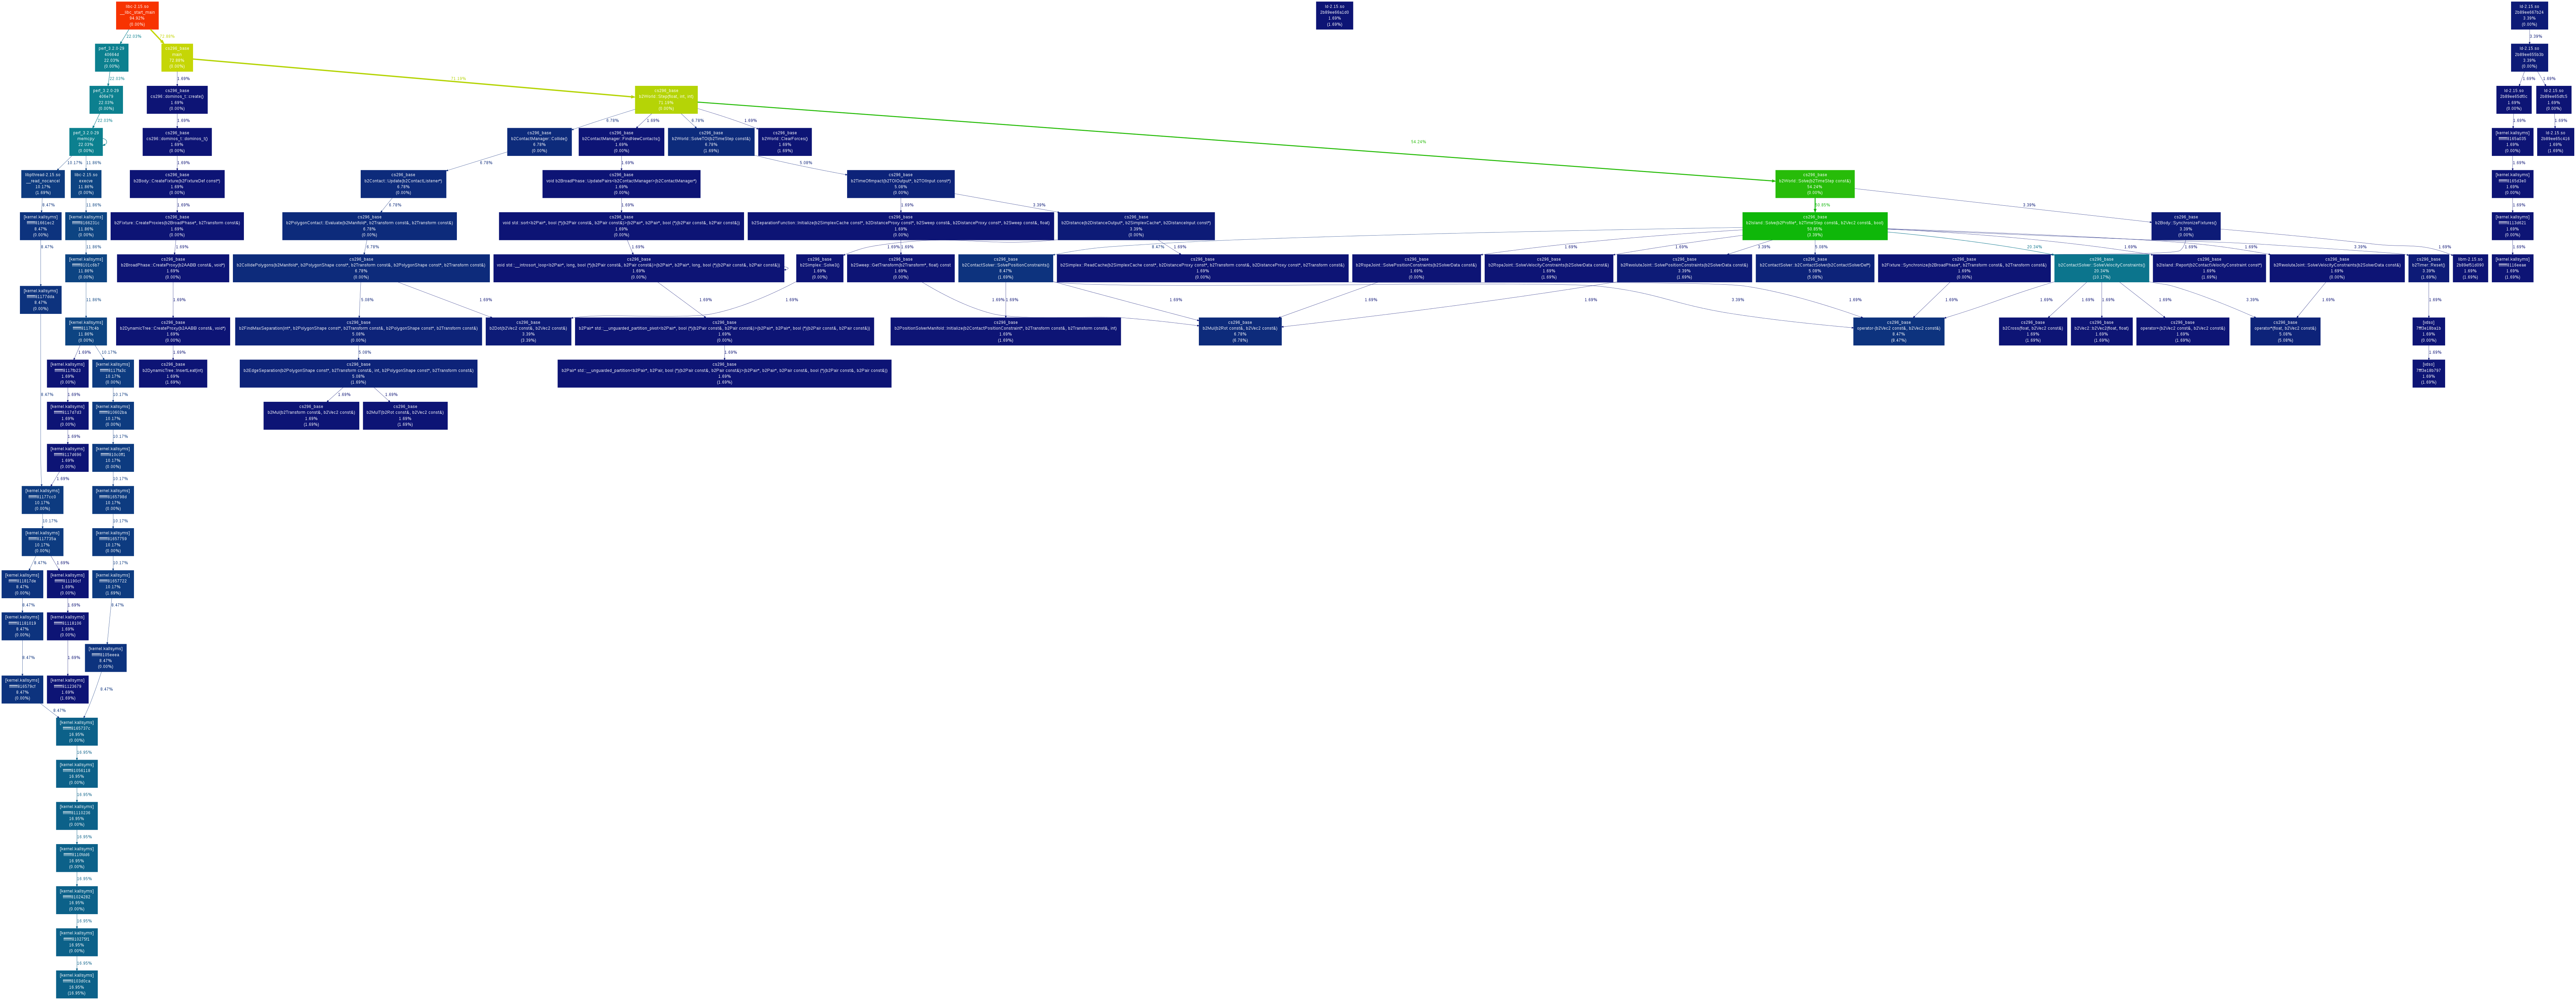
\includegraphics[scale=0.1]{./doc/deb_output200.png}
\begin{center}
Fig.9 : Call Graph for Debug Mode:Itr value 200
\end{center}
\end{center}

\begin{center}
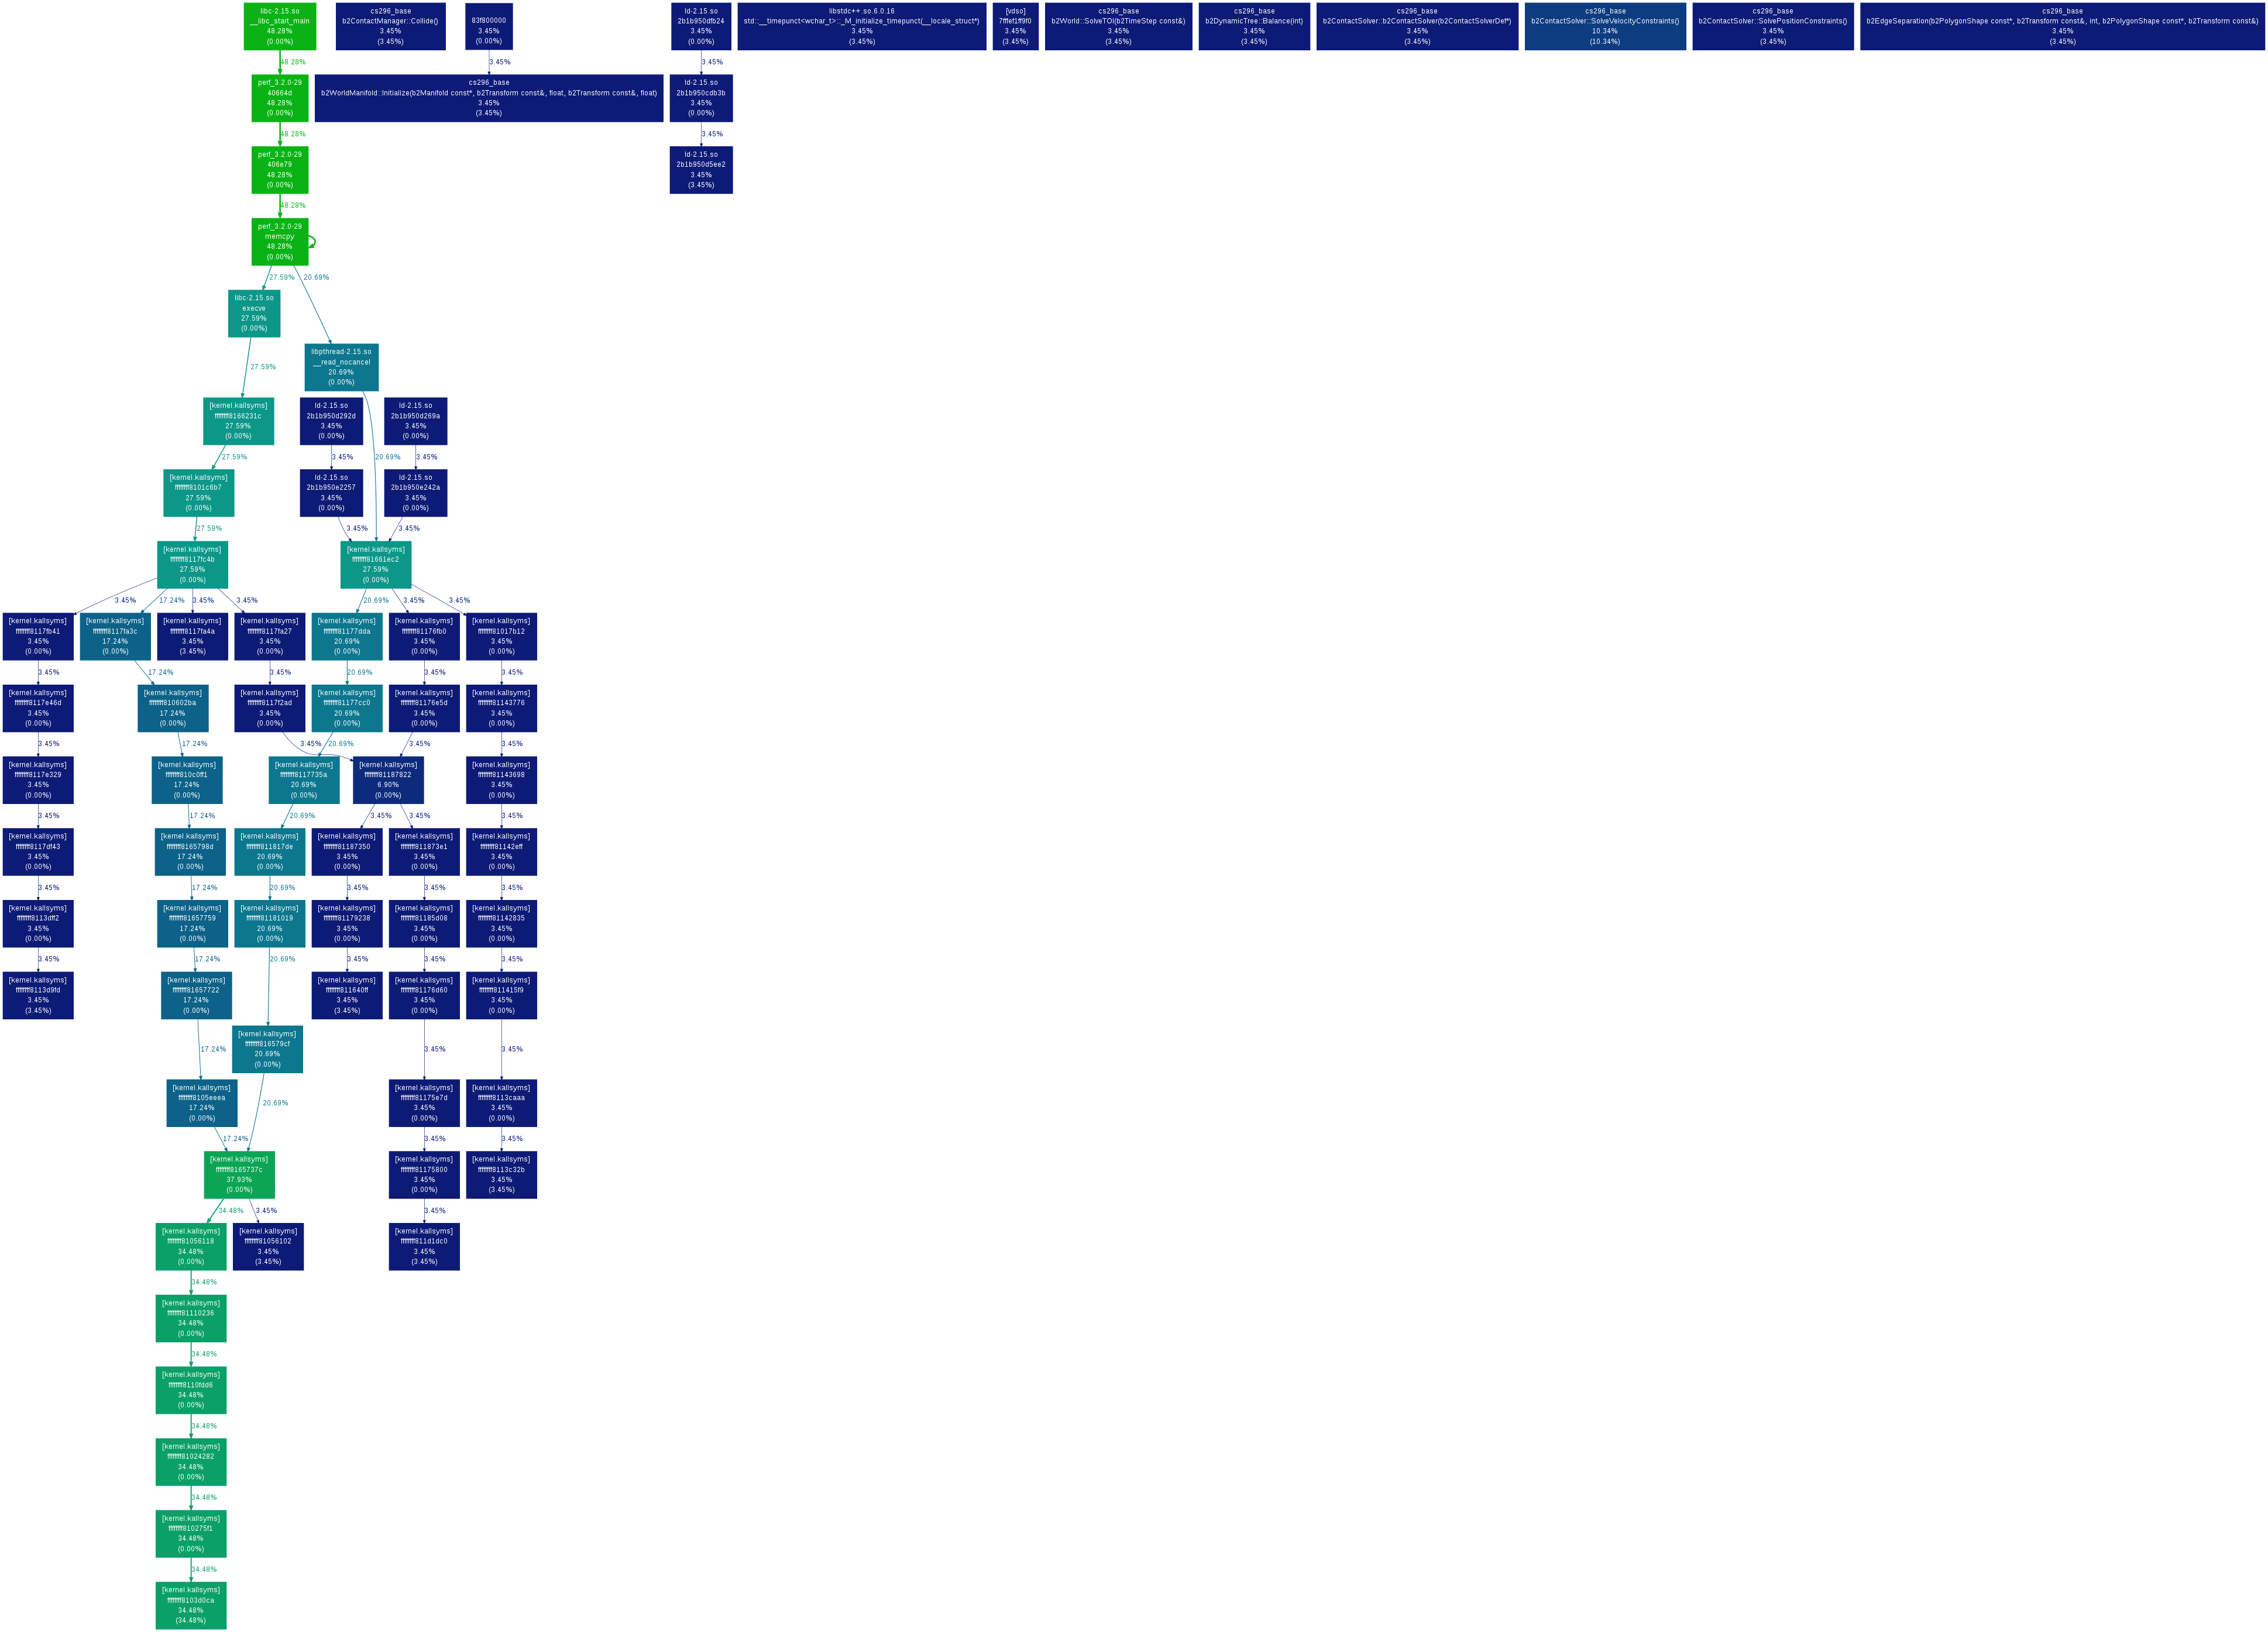
\includegraphics[scale=0.1]{./doc/rel_output200.png}
\begin{center}
Fig.10 : Call Graph for Release Mode:Itr value 200
\end{center}
\end{center}

\subsection{Conclusion}
\begin{itemize}
\item{We can see that number of functions calls for constructors are reduced drastically in the release part as compared to debug part and hence indicates that optimization flags work on constructors.}

\item{Here is a consistent observation. Most of the time is taken by method "b2ContactSolver::SolveVelocityConstraints()". Hence there is a possiblity of implementation optimization of this function in Box2D Library.}
\end{itemize}

\section{Conclusion}
Thus in the report we have analyzed and timed the code under different conditions and summerized the results.


\bibliographystyle{plain}
\bibliography{./doc/referredto}{}
\end{document}
